\documentclass[hyperref]{ctexart}
\usepackage[left=2.50cm, right=2.50cm, top=2.50cm, bottom=2.50cm]{geometry} %页边距
\usepackage{helvet}
\usepackage{amsmath, amsfonts, amssymb} % 数学公式、符号
\usepackage[english]{babel}
\usepackage{graphicx}   % 图片
\usepackage{url}        % 超链接
\usepackage{bm}         % 加粗方程字体
\usepackage{multirow}
\usepackage{booktabs}
\usepackage{algorithm}
\usepackage{algorithmic}
\usepackage{fancyhdr} %设置页眉、页脚
\pagestyle{fancy}
\lhead{}
\chead{}
\lfoot{}
\cfoot{}
\rfoot{}
\usepackage{hyperref} %bookmarks
\hypersetup{colorlinks, bookmarks, unicode} %unicode
\usepackage{multicol}
\title{\textbf{半导体探测器与$\alpha$粒子能损实验}}
\author{\sffamily 赵宇航}
\date{}
\begin{document}
\maketitle
\indent{\bf 摘要: }本实验以放射源$^{241}Am$放射源分别通过1-7层铝箔和Mylar膜,测量了通过后的粒子能量,借以拟合了单层铝箔和Mylar膜的厚度。\\	
\begin{multicols}{2}
\CTEXsetup[format={\Large\bfseries}]{section}
	\section{实验目的}
	1.了解$\alpha$粒子通过物质时的能量损失及其规律。

	2.学习从能损测量求薄箔厚度的方法。
	\section{实验原理}
	天然放射性物质放出的$\alpha$粒子,能量范围是$3-8MeV$。在这个能区内,$\alpha$粒子的核反应截面很小,因此可以忽略。$\alpha$粒子与原子核之间虽然有可能产生卢瑟福散射,但几率较小。它与物质的相互作用主要是与核外电子的相互作用。$\alpha$粒子与电子碰撞,将使原子电离、激发而损失其能量。在一次碰撞中,具有质量为$m$,能量为$E$的带电粒子,转移给电子(质量为 $m_0$)的最大能量约为 $\frac{4Em_0}{m}$,$\alpha$粒子的质量比电子大得多,所以每碰撞一次,只有能量的一小部分转移给电子。当它通过吸收体时,经过多次碰撞后,才损失较多能量。每一次碰撞后,$\alpha$粒子的运动方向基本上不发生偏转,因而它通过物质的射程几乎接近直线。带电粒子在吸收体内单位路程上的能量损失即能量损失率$-\frac{dE}{dx}$,称为线性阻止本领$S$.
	\begin{equation}
	S=-\frac{dE}{dx}
	\end{equation}

	它的单位是$erg/cm$,实用上常换算成KeV/$\mu m$ 或$eV/μg ·{cm}^2$ 。把 S 除以吸收体单位体积内的原子数$N$,称为阻止截面,用$\sum_e$ 表示,并常取 eV/${10}^{15}$atom·${cm}^2$为单位。
	\begin{equation}
	\Sigma_e=-\frac1 N \frac{dE}{dx}\label{11}
	\end{equation}
	
	对非相对论性$\alpha$粒子($v\ll c$),线性阻止本领用下面式子表示:
	\begin{equation}\label{AA}
	-\frac{dE}{dx}=\frac{4\pi z^2e^4NZ}{m_0v^2}ln\frac{2m_0v^2}{I}
	\end{equation}

	\eqref{AA}式中的$z$为入射粒子的电荷数,$Z$为吸收体的原子序数,$e$为电子的电荷,$v$为入射粒子的速度,$N$为单位体积内的原子数,$I$是吸收体中的原子的平均激发能。\eqref{AA}式中,对数项随能量的变化是缓慢的,因此\eqref{AA}式可近似表示为
	\begin{equation}
	\frac{dE}{dx}\propto -\frac{C}{E}
	\end{equation}

	$C$为一常数。

	当$\alpha$粒子穿过厚度为$\triangle X$ 的薄吸收体后,能量由 $E_1$变为$ E_2$,可以写成
	\begin{equation}\label{BB}
	\triangle E=E_1-E_2=-(\frac{dE}{dx})_{ave}\triangle X 
	\end{equation}

	$(\frac{dE}{dx})_{ave}$是平均能量$\frac{E1+E2}{2}$ 的能量损失率。这样测定了$\alpha$粒子在通过薄箔后的能量损失$\triangle$E,则利用\eqref{BB}式,可以求薄箔的厚度,即
	\begin{equation}\label{CC}
	\triangle X=\frac{\triangle E}{-(\frac{dE}{dx})_{ave}} \approx \frac{\triangle E}{-(\frac{dE}{dx})_{E_1}}
	\end{equation}

	当$\alpha$粒子能量损失比较小时,\eqref{CC}式中的阻止本领可用入射能量$E1$时之值;当箔比较厚时,$\alpha$粒子的能量在通过箔后能量损失大时,\eqref{CC}式就应表为
	\begin{equation}\label{DD}
	\triangle X=\int^{E_1}_{E_2}\frac{dE}{-\frac{dE}{dx}}\approx \sum^{E_1}_{E_2}\frac{\delta E}{(-\frac{dE}{dx})_{E_1}}
	\end{equation}
	
	\eqref{DD}式中$\delta E$可取$10keV$,在这范围内,将$S$看作常量。

	\begin{center}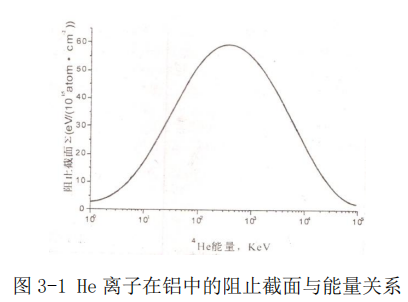
\includegraphics[scale=0.5]{HeAl.png}\end{center}
	图表示$^{4}He$离子在铝中的阻止截面与能量关系的实验结果。能量在$1KeV —10MeV$之间的$^{4}He$离子在铝中的阻止截面,可用曲线拟合得到的经验公式表示为

	\begin{equation}
	{\sum}_e=\frac{A_1E^{A_2}(\frac{A_3}{E/1000}ln[1+\frac{A_4}{E/1000}+\frac{A_5E}{1000}])}{A_1E^{A_2}+\frac{A_3}{E/1000}ln[1+\frac{A_4}{E/1000}+\frac{A_5E}{1000}]}\label{chang}
	\end{equation}

	式中的$A1$、$A2$、$A3$、$A4$、$A5$为常数,见表$1$。$^{4}He$离子的能量以$keV$为单位,得到$\sum_e$ 以$eV/10^{15} atom\cdot{cm}^2$为单位。对于化合物,它的阻止本领可由布拉格相加规则,将化合物的各组成成份的阻止本领 $(\frac{dx}{dE})_i$ 相加得到,即
	\begin{equation}
	({-\frac{dE}{dx}})_e=\frac{1}{A_e}\sum Y_iA_i({-\frac{dE}{dx}})_i(KeV/\mu g{cm}^{-2})\label{fuhe}
	\end{equation}

	\begin{center}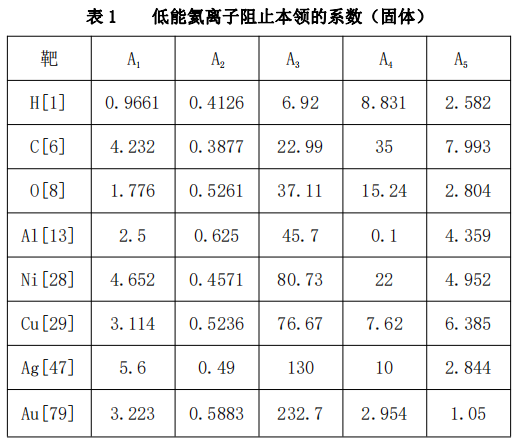
\includegraphics[scale=0.45]{biao1.png}\end{center}
	其中$ Y_i$、$A_i$分别为化合物分子中的第$i$种原子的数目、原子量,$A_e$(等于$\sum Y_iA_i$)是化合物的分子量。利用已知的阻止截面,通过$\alpha$粒子在薄箔中能损的测量,可以快速无损的测定薄箔的厚度,$\alpha$粒子的能量可用多道分析器测量,峰位可按最简单的重心法得到。
	\section{实验结果}
	将测量的$^{241}Am$\hspace{0.5em} $\alpha$谱以多道的道数为横坐标,以计数为纵坐标描绘在坐标纸上,如下图所示
	\begin{center}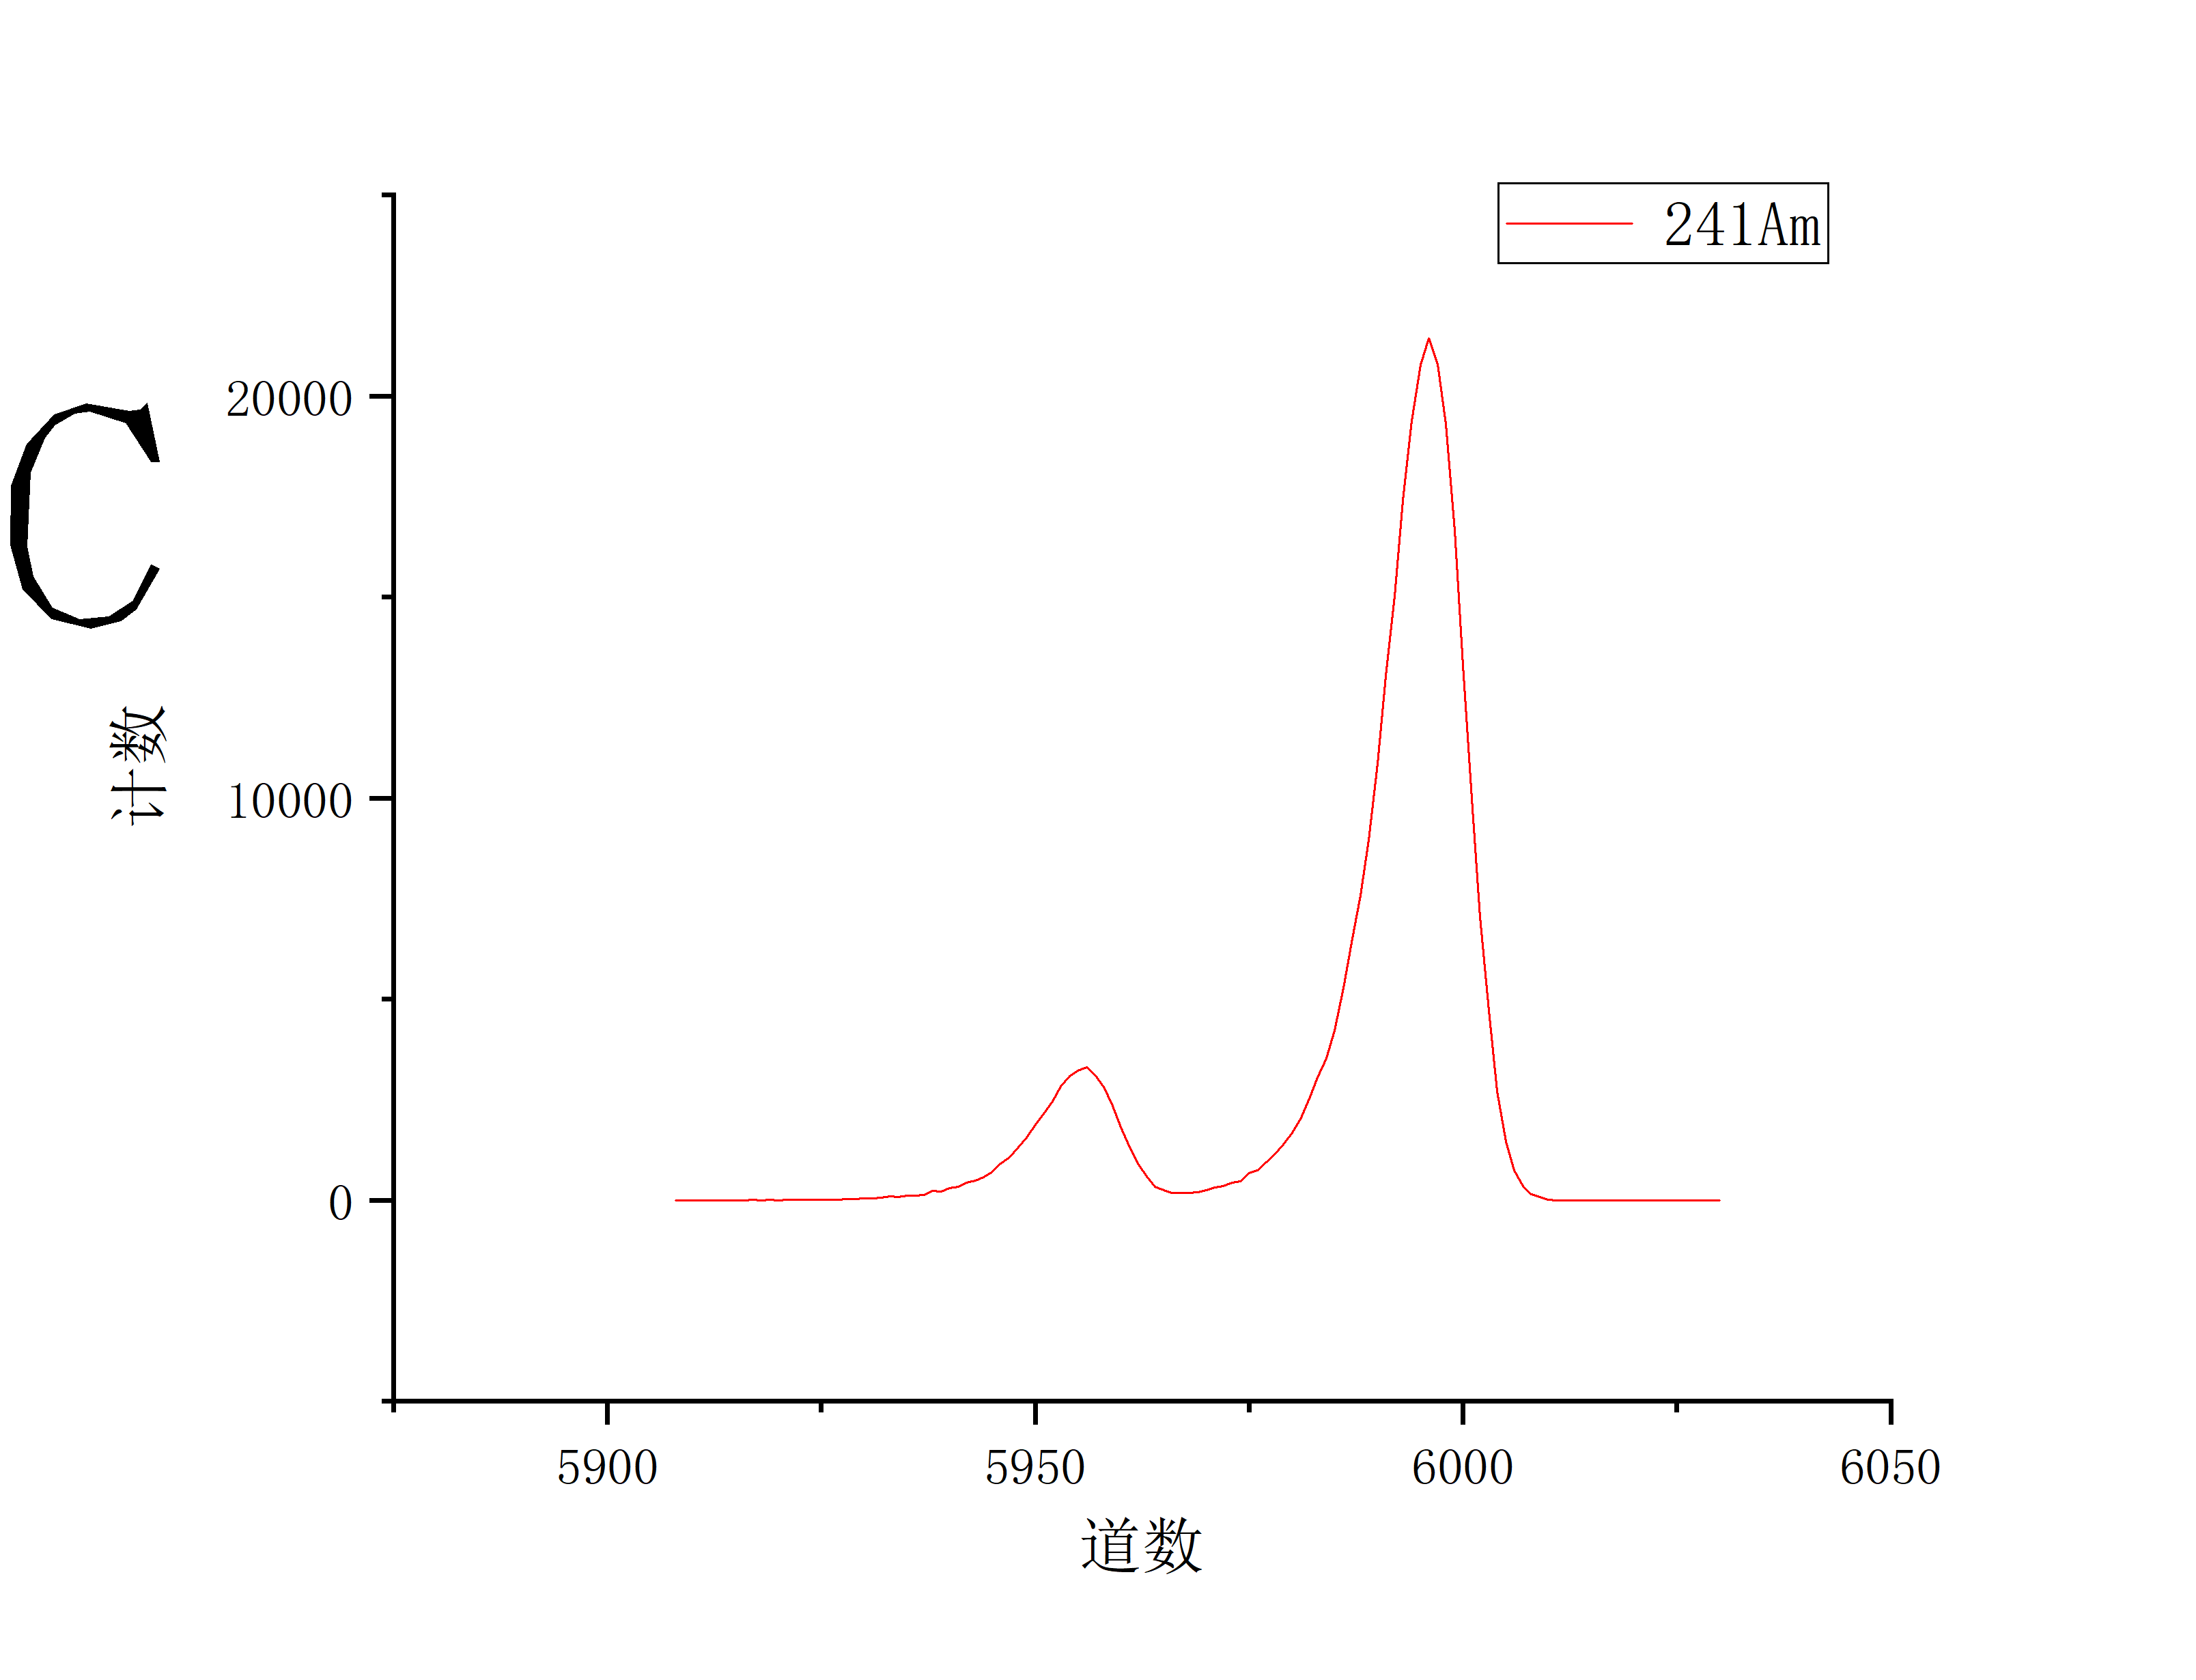
\includegraphics[scale=0.3]{T1.png}\end{center}
	结合图形由实验数据知其峰值处能量分别为$5954.79keV,5995.23keV$,半高宽分别为$11.8899keV,11.5963keV$。由能量分辨率定义知两个峰能量分辨率分别为$0.1997\%,0.1934\%$。

	根据实际实验情况,我们以放射源$^{241}Am$、$^{239}Pu$、$^{244}Cm$放射源的能量为横坐标,以全能峰道址为纵坐标在坐标纸上作出校准曲线,如图所示。
	\begin{center}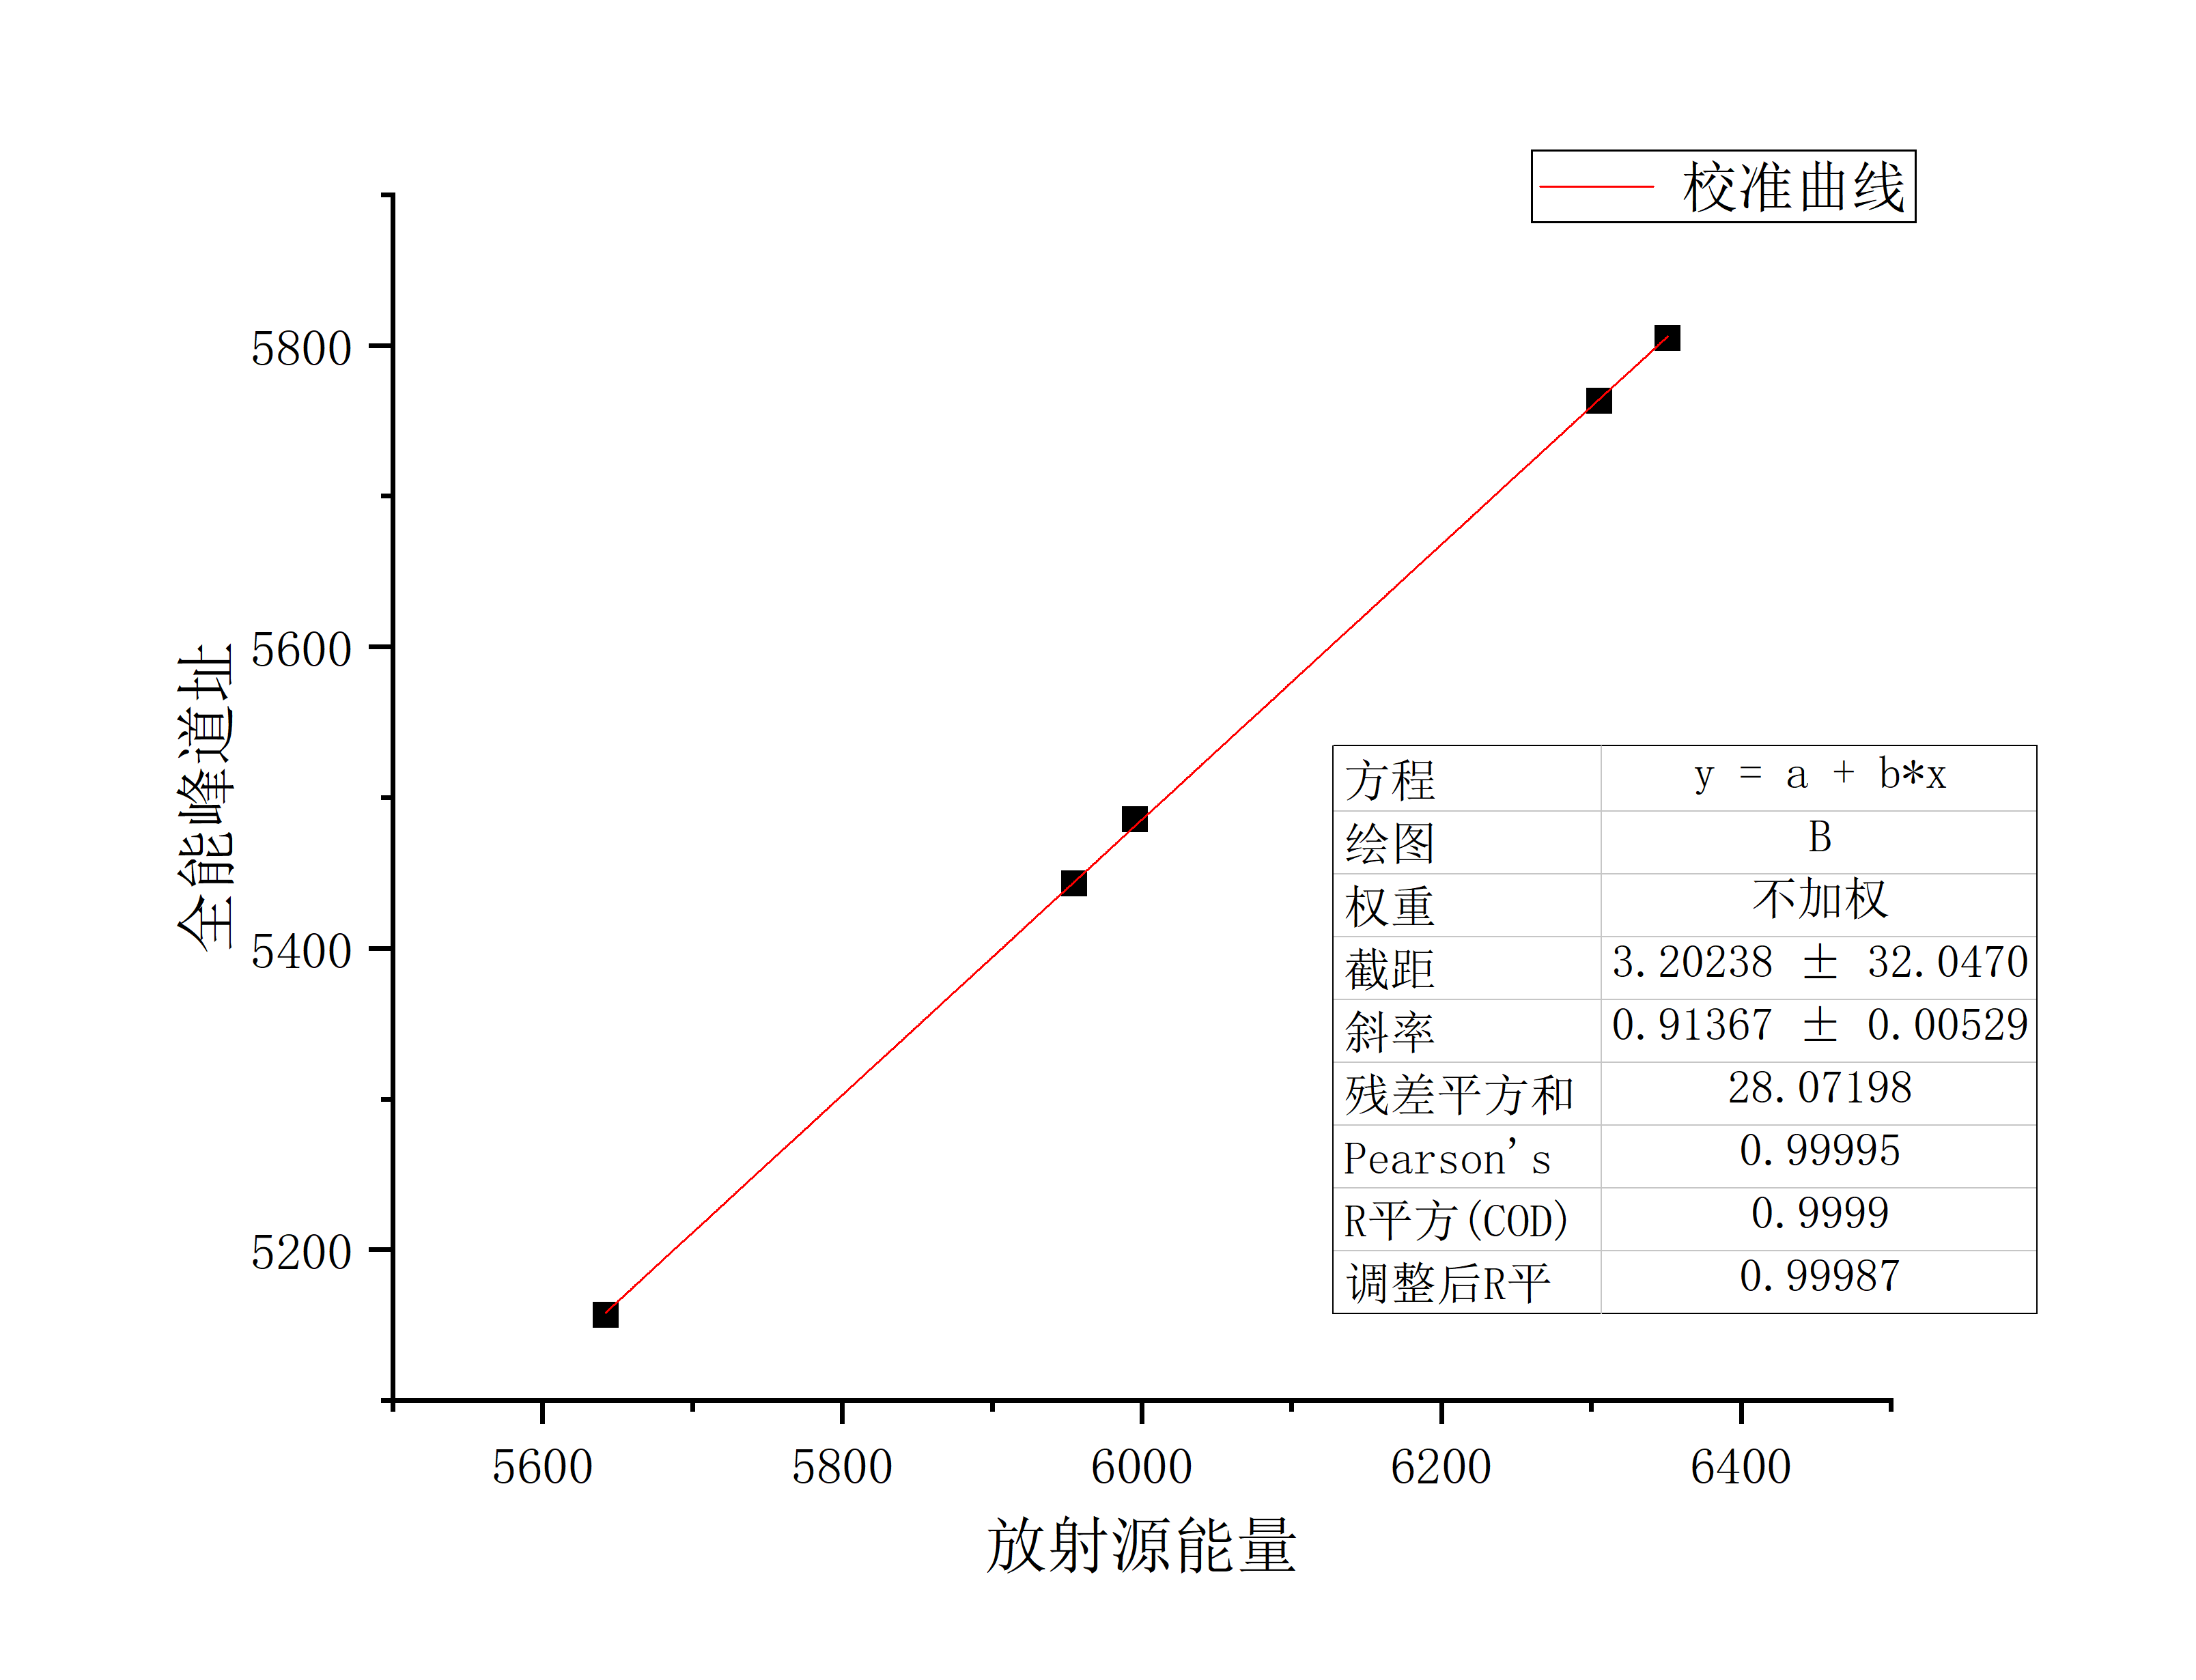
\includegraphics[scale=0.3]{T2.png}\end{center}

	\subsection{Al的相关处理}
	利用式\eqref{chang},可以求得${\sum}_e=25.53 eV/10^{15} atom\cdot{cm}^2$,由$N=\frac{\rho}{M}N_A$得$N=6.02\times 10^{22}/cm^2$,再利用式\eqref{11}可得$(\frac{dE}{dx})_{ave}=153.69KeV/\mu m$。

	利用之前的校准曲线可得$\alpha$通过1-7层铝的能量依次为5166.53,4835.75,4488.17,4119.56,3724.91,3294.63,2825.76$(KeV)$。
利用式\eqref{CC}求得铝箔厚度依次为2.076049815,4.228337451,6.489892148,8.888298191,11.45613357,14.25576018,17.3064989。
以铝箔层数为横坐标,厚度为纵坐标,线性拟合结果如下图所示,可知铝箔单片厚度为$2.5\mu m$。
	\begin{center}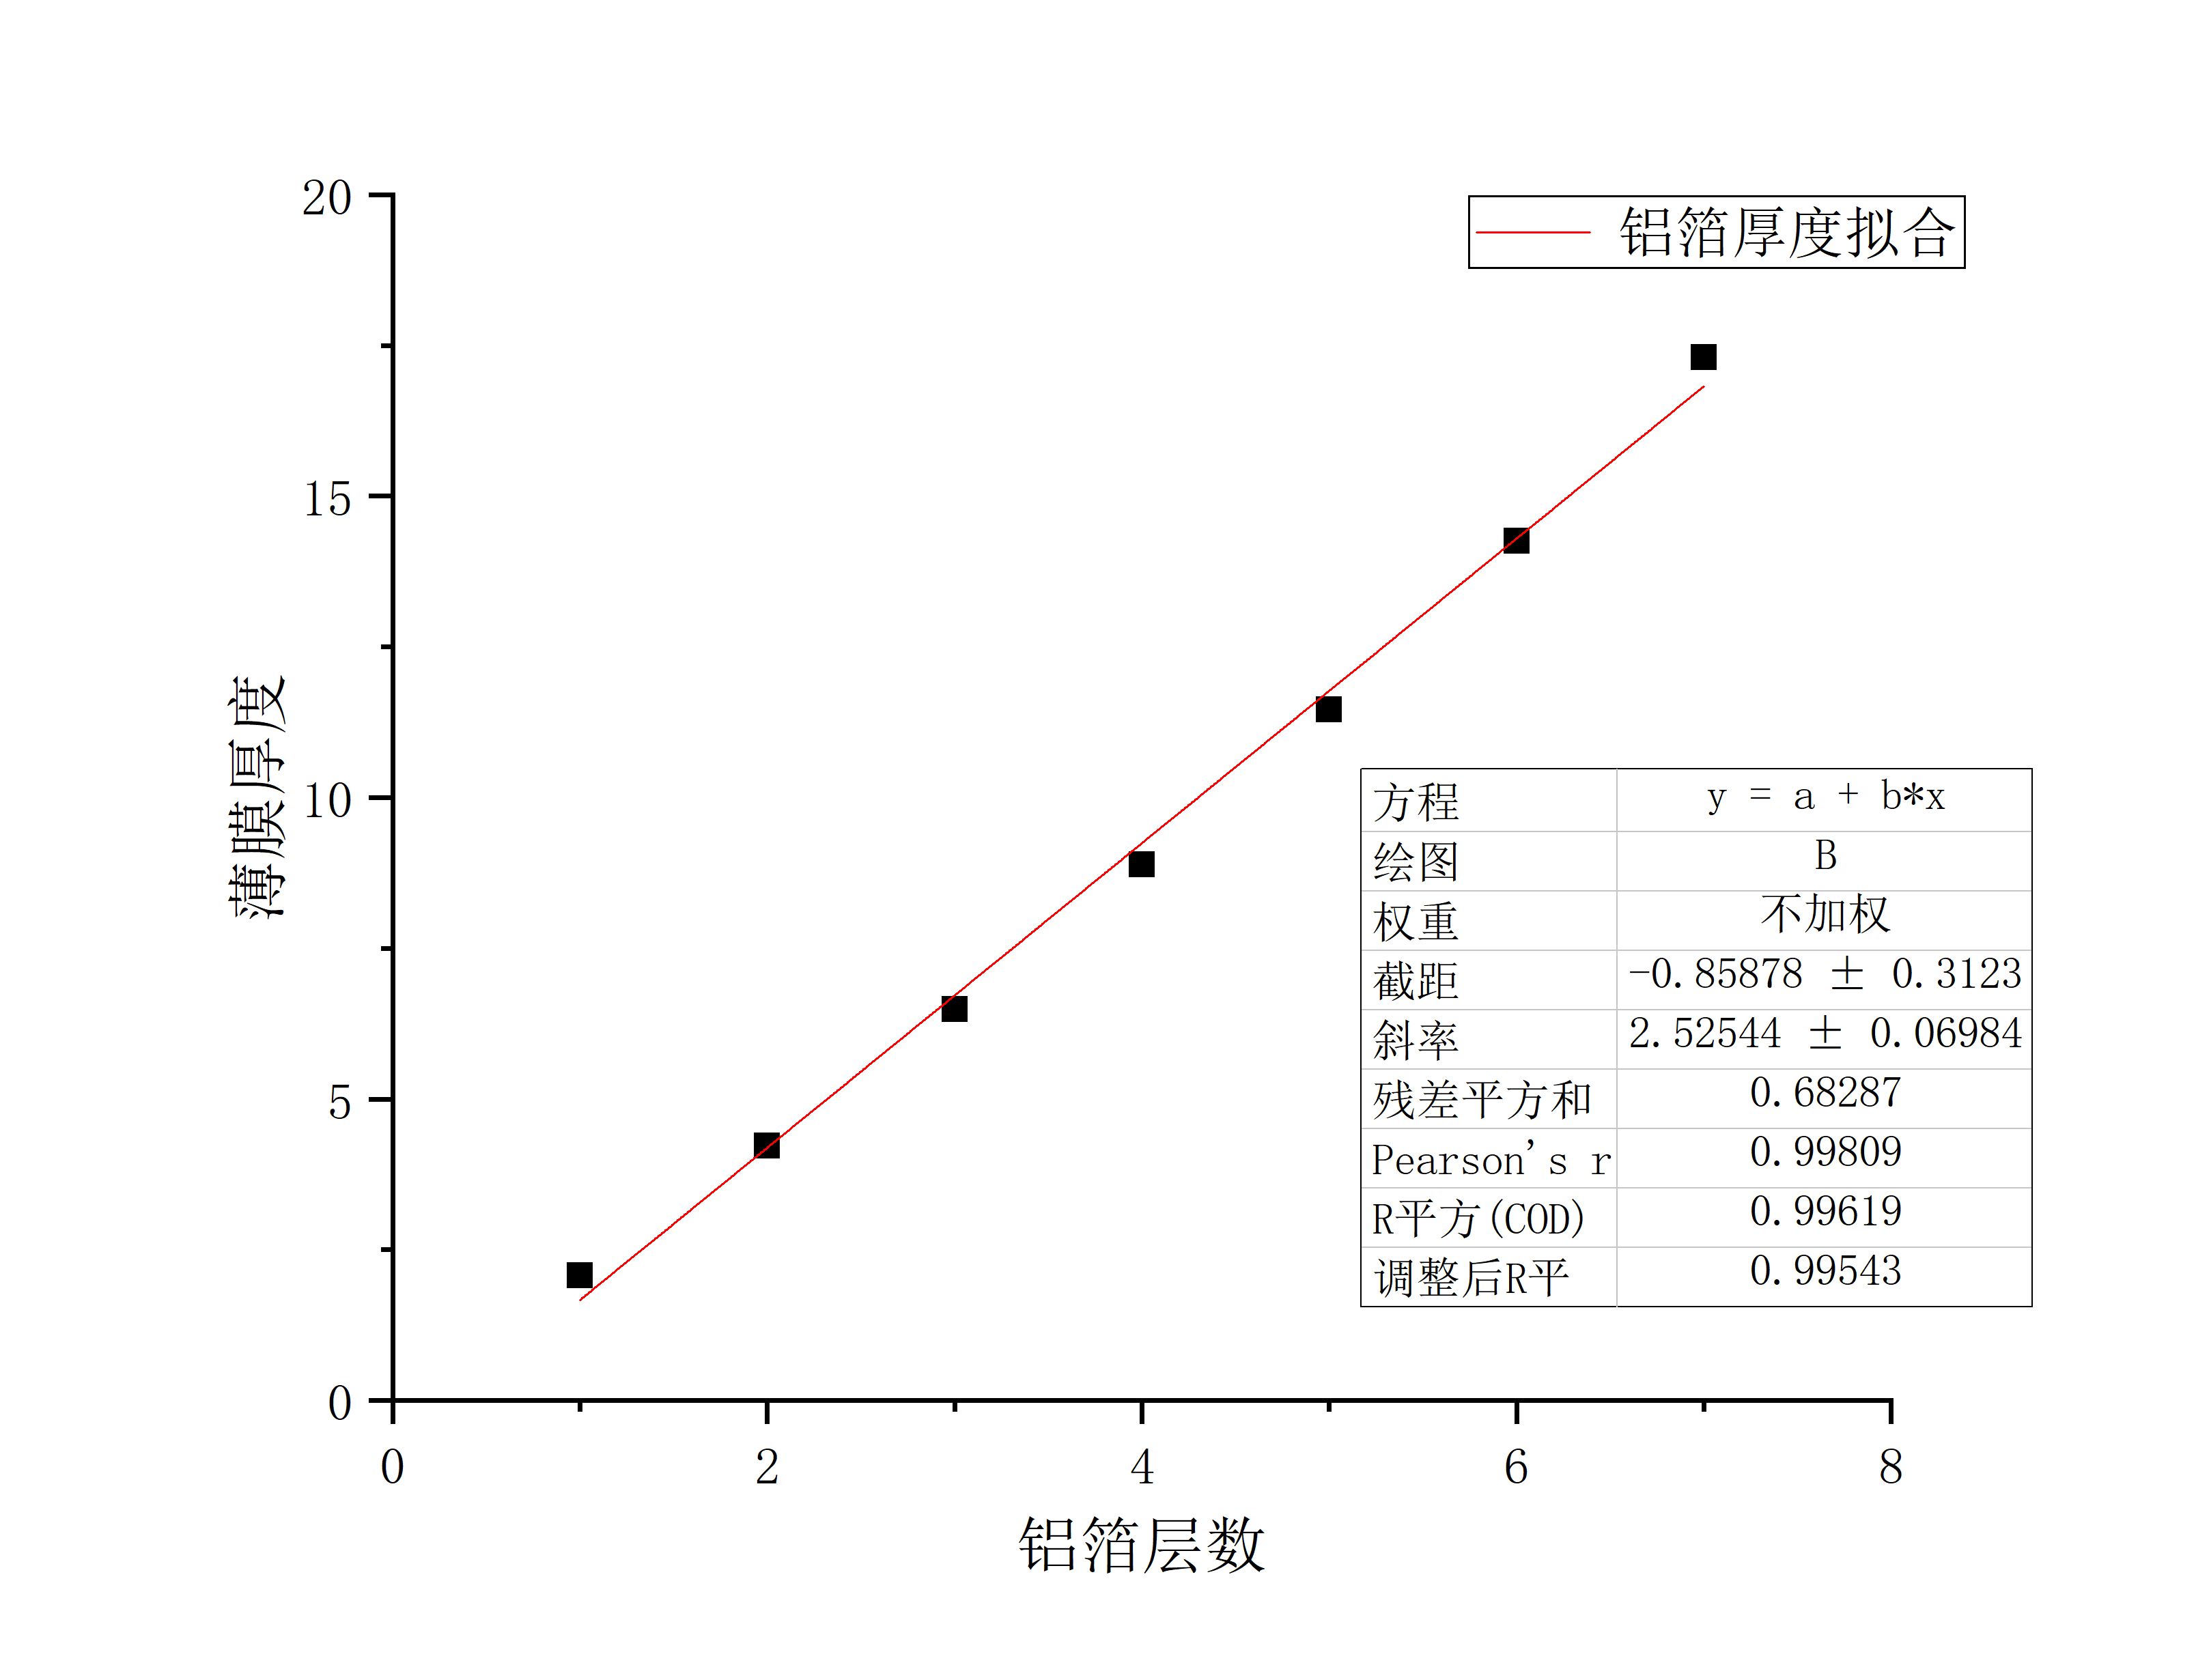
\includegraphics[scale=0.3]{T3.png}\end{center}

	\subsection{Mylar的相关处理}
	取Mylar为$C_{10}H_8 O_1$,仿照铝的过程,利用式\eqref{chang}分别计算$${\sum}_C=14.49 eV/10^{15} atom\cdot{cm}^2$$ 
$${\sum}_H=3.22 eV/10^{15} atom\cdot{cm}^2$$ $${\sum}_O=17.81 eV/10^{15} atom\cdot{cm}^2$$
取$$N(C)=1.136\times10^{23}atm\cdot cm^{-3}$$ $$N(H)=5.376\times10^{19}atm\cdot cm^{-3}$$ $$N(O)=5.367\times10^{19}atm\cdot cm^{-3}$$ 
进而求得$$(\frac{dE}{dx})_{C}=164.606KeV/\mu m$$ $$(\frac{dE}{dx})_{H}=0.017KeV/\mu m$$ $$(\frac{dE}{dx})_{O}=0.096KeV/\mu m$$
利用\eqref{fuhe},可以求得$$(\frac{dE}{dx})_{ave}=129.96KeV/\mu m$$

	仿照铝的过程,可得$\alpha$通过1-7层Mylar薄膜的能量依次为5196.7,4898.04,4585.36,4254.78,3900.04,3510.96,3097.74$(KeV)$。
利用式\eqref{CC}求得Mylar膜厚度依次为2.186903663,4.484995383,6.890966451,9.434672207,12.16428132,15.15812558,18.3377193。
以Mylar膜层数为横坐标,厚度为纵坐标,线性拟合结果如下图所示,可知Mylar膜单片厚度为$2.7\mu m$。
	\begin{center}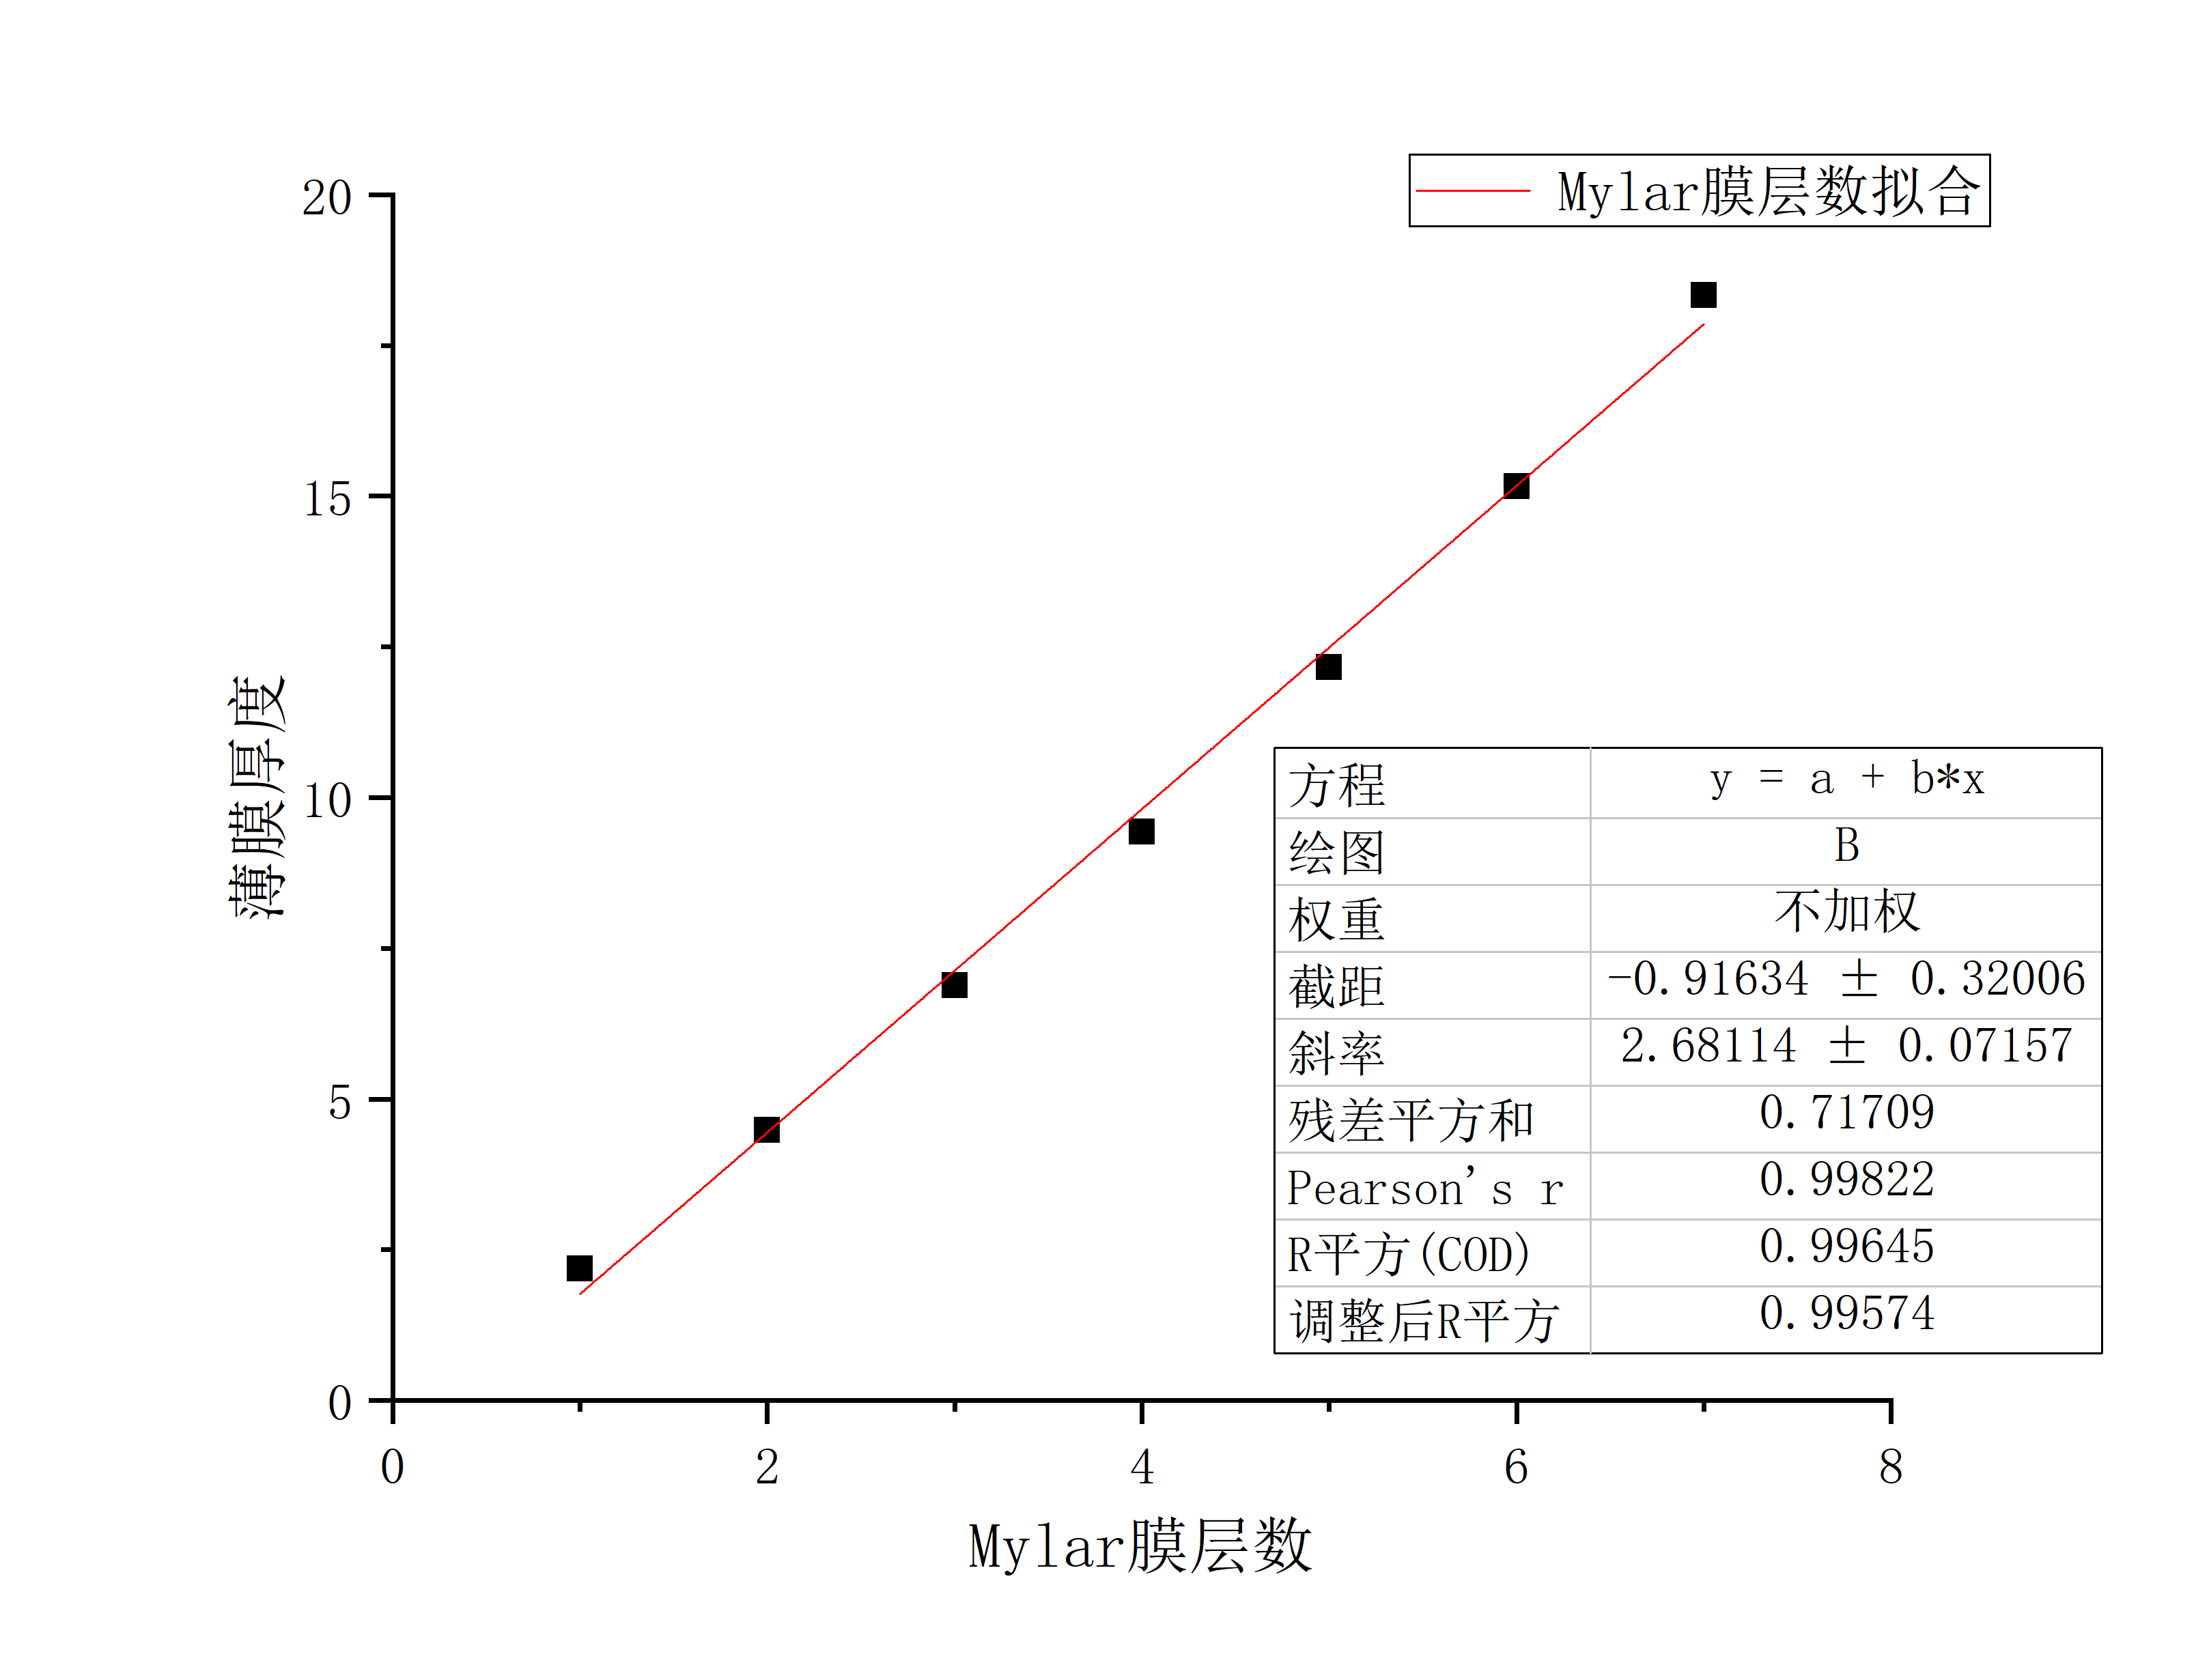
\includegraphics[scale=0.3]{T4.png}\end{center}

	\section{结论与讨论}
	$\alpha$粒子和其他粒子碰撞时,有可能向各个方向散射,能量的变化幅度就增大。穿过更厚的薄片,发生碰撞的次数增加,能量的变化幅度变得更大。所以$\alpha$粒子穿过吸收体后能谱展宽,且穿过的吸收体更厚,展得越宽。

	注意到,$\triangle E=-(\frac{dE}{dx})_{ave}\triangle X ^{'}=S\frac{\triangle X}{cos \theta}$。当入射角与表面法线
交角为$4^{\circ}$时,$\triangle E=S\frac{\triangle X}{cos (\frac{\pi}{45})} \approx 1.0024S\triangle X$;当入射角与表面法线交角为$6^{\circ}$时,$\triangle E=S\frac{\triangle X}{cos (\frac{\pi}{30})} \approx 1.0055S\triangle X$。

	仿照铝的处理,利用金的密度$\rho=19.31g/cm^{3}$和阻止本领$(\frac{dE}{dx})_{ave}=0.228KeV/(\mu g \cdot cm^{-2})$可得$(\frac{dE}{dx})_{ave}=440.27KeV/\mu m$。结合式\eqref{BB}知$\triangle X=4.4KeV$,取$^{241}Am$能量为$5485.6KeV$,到灵敏区为$5481.2KeV$。

	在3.2节,我们已经处理了这个题目,Mylar膜单片厚度为$2.7\mu m$。

	在3.1节,我们有$N=6.02\times 10^{22}/cm^2$。取穿过0-7片铝箔能量近似为5480,5170,4840,4490,4120,3720,3300,2830$(KeV)$。由式\label{DD}分$0-i(i\in \{1,2,3,4,5,6,7\})$片薄膜取7个间隔分别算得$\triangle X=$2.0428,4.0674,6.1231,8.1928,10.3097,12.3964,14.5648。
以铝箔层数为横坐标,厚度为纵坐标,线性拟合结果如下图所示,可知铝箔单片厚度为$2.1\mu m$。
	\begin{center}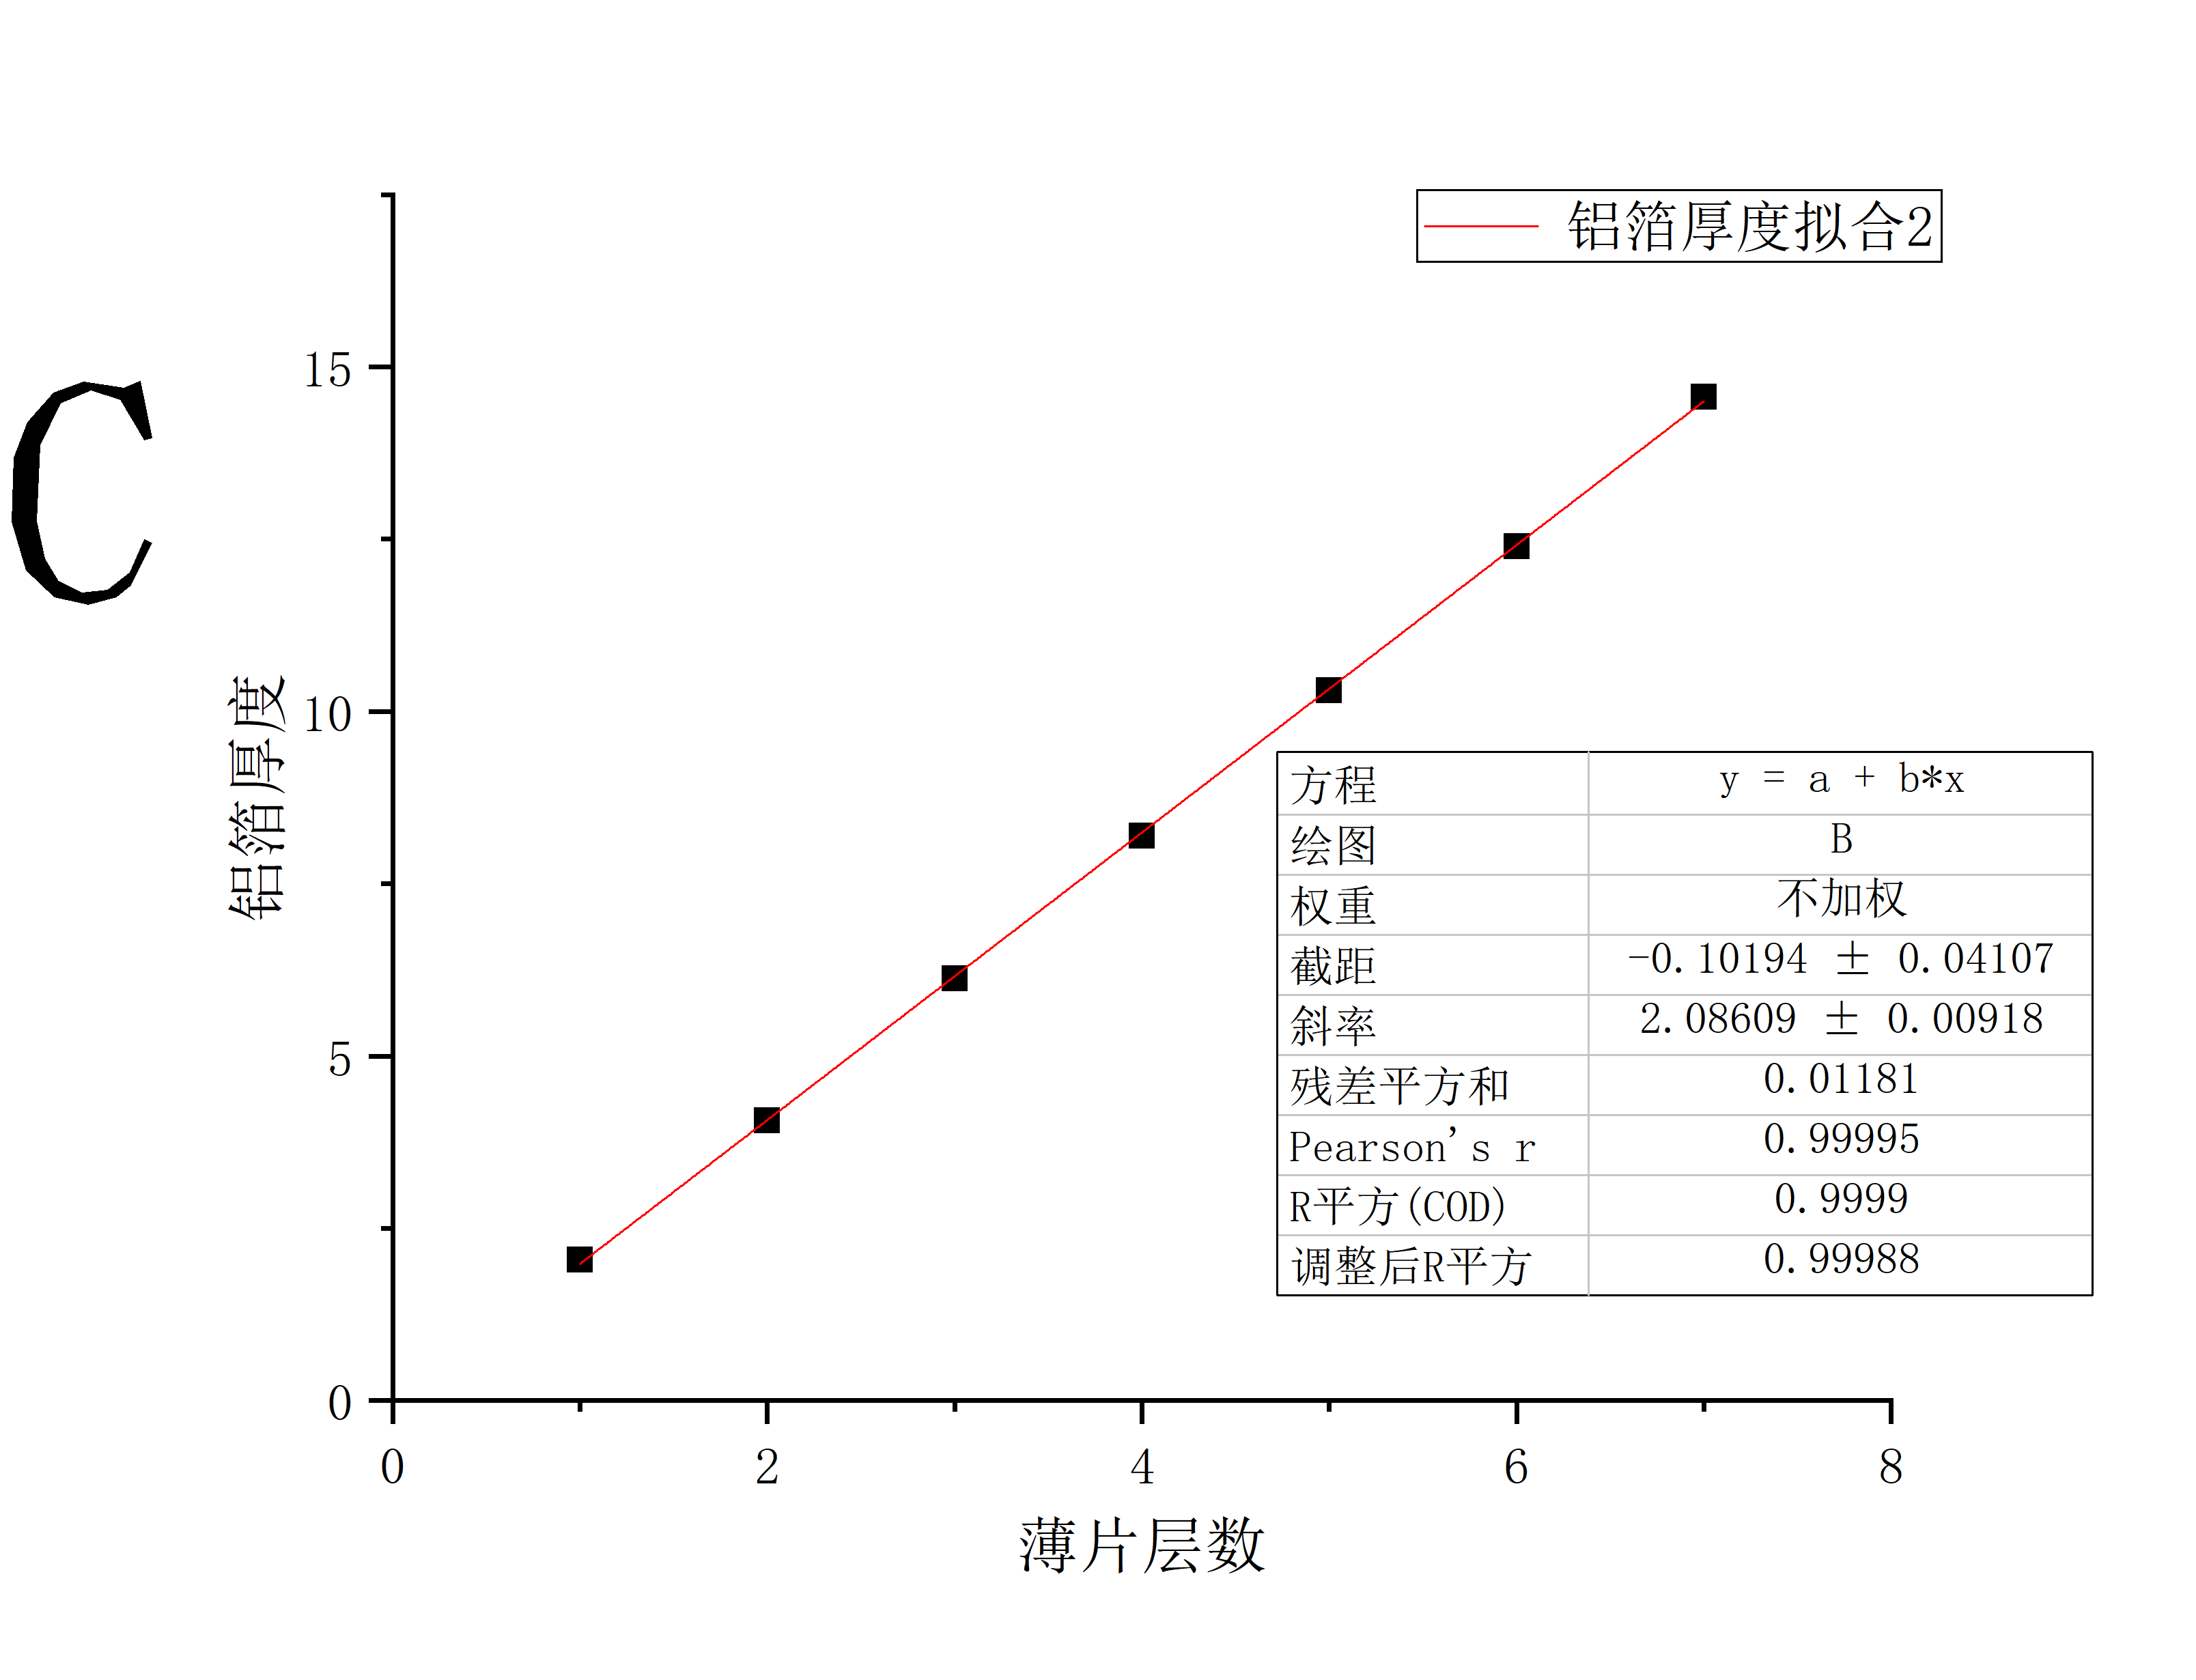
\includegraphics[scale=0.3]{sk.png}\end{center}

	由此可见,我们之前求的铝箔单片厚度偏大。如果不全部使$E_0$作为${\sum}_e$基能量会更贴近一些,应该和计算出$1$片铝箔相当,即$2.076\mu m$左右。但对我们的实验设施,这个精度已经够了。
\end{multicols}
\end{document}